\section{Wstep}
\subsection{Opis dziedziny przedmiotowej}
Dziedziną projektu jest grafika, w~głównej mierze operację cyfrowe. 
\subsection{Cel projektu – po co?}
Celem projektu jest zrealizowanie programu umożliwiającego cyfrowe przetwarzanie obrazu, jako z wizualizowanego ciągu bloków, na każdym z nich będzie dodana możliwość poglądu obrazu w~każdym jego stadium przekształcania. Użytkownik będzie mógł dodawać własne typy danych jaki i funkcji operujących na nich. 
\subsection{Zakres projektu – co i jak?}
\begin{enumerate}
\item stworzenie dokumentacji
\item zrealizowanie graficznego interfejsu
\item implementacja operacji przetwarzania obrazu takich jak: \\
(wybór pozostawiony dla pozostałych osób z grupy)
\item dodanie opcji tworzenia własnych dodatków (plug-in)
\end{enumerate}
\subsection{Opracowanie wymagań wstępnych}
\subsubsection{Oczekiwana funkcjonalność systemu}
Możliwość:
\begin{enumerate}
 \item tworzenia bloków reprezentujących wybrane operacje cyfrowe.
 \item tworzenie własnych dodatków.
 \item wczytania różnych formatów obrazów.
 \item zapis powstałych obrazów.
 \item zapis aktualnego stanu programu (położenia i połączeń bloków).
\end{enumerate}
\subsubsection{Opis rzeczywistych obiektów i zależności między nimi}

\subsubsection{Ograniczenia (system, środowisko, specyficzne wymagania)}
Program zostanie napisany w IDE Borland C++, darmowa biblioteka FreeImage umożliwi wczytywanie wielu formatów plików.
\subsection{Harmonogram prac}
\begin{enumerate}
 \item Stworzenie dokumentacji projektu - Piotr Wilk
 \item Zaprojektowanie oraz Implementacja silnika aplikacji - Piotr Zegar, Piotr Wilk
 \item Implementacja GUI - Piotr Zegar
 \item Pisanie wtyczek - pozostałe osoby.
\end{enumerate}
\section{Podział projektu}
\subsection{Engine}
\begin{figure}[h]
 \centering
 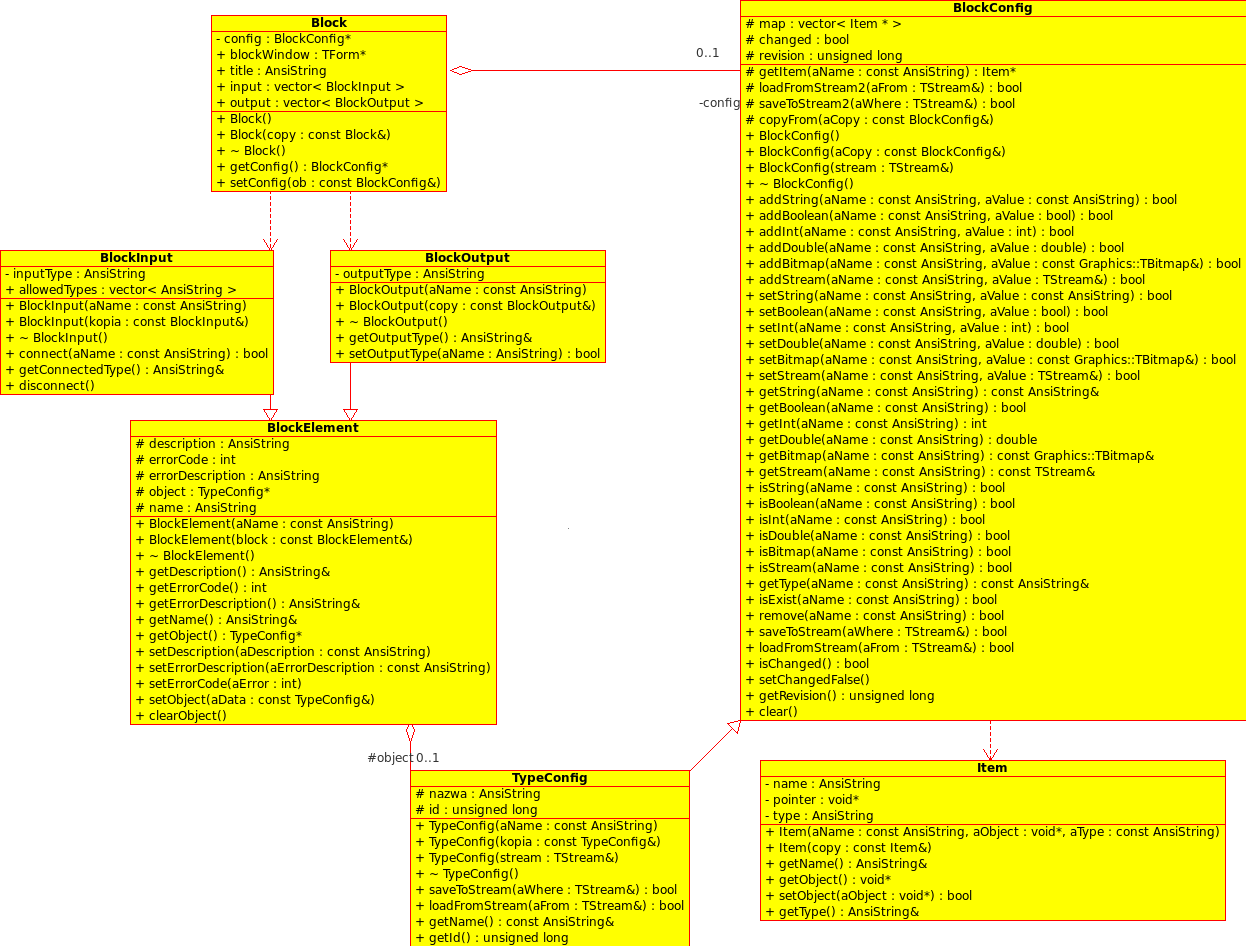
\includegraphics[scale=0.4]{diagram-engine.png}
 \caption{Engine - diagram}
 \label{fig:engine}
\end{figure}
\newpage
\subsection{BRIGE}
\begin{figure}[h]
 \centering
 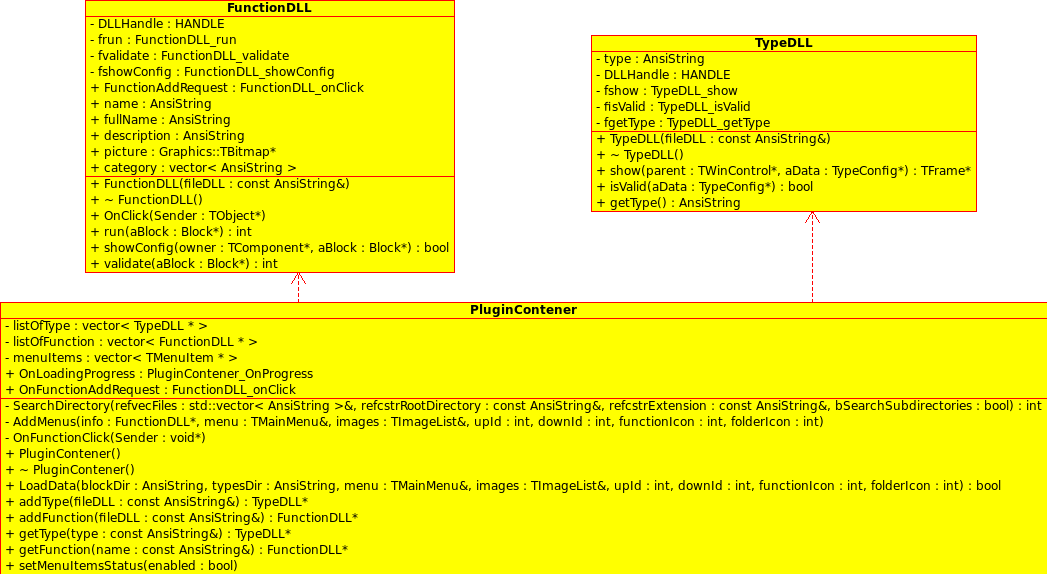
\includegraphics[scale=0.4]{diagram-brige.png}
 \caption{Engine - BRIGE}
 \label{fig:brige}
\end{figure}
\newpage
\subsection{GUI}
\begin{figure}[h]
 \centering
 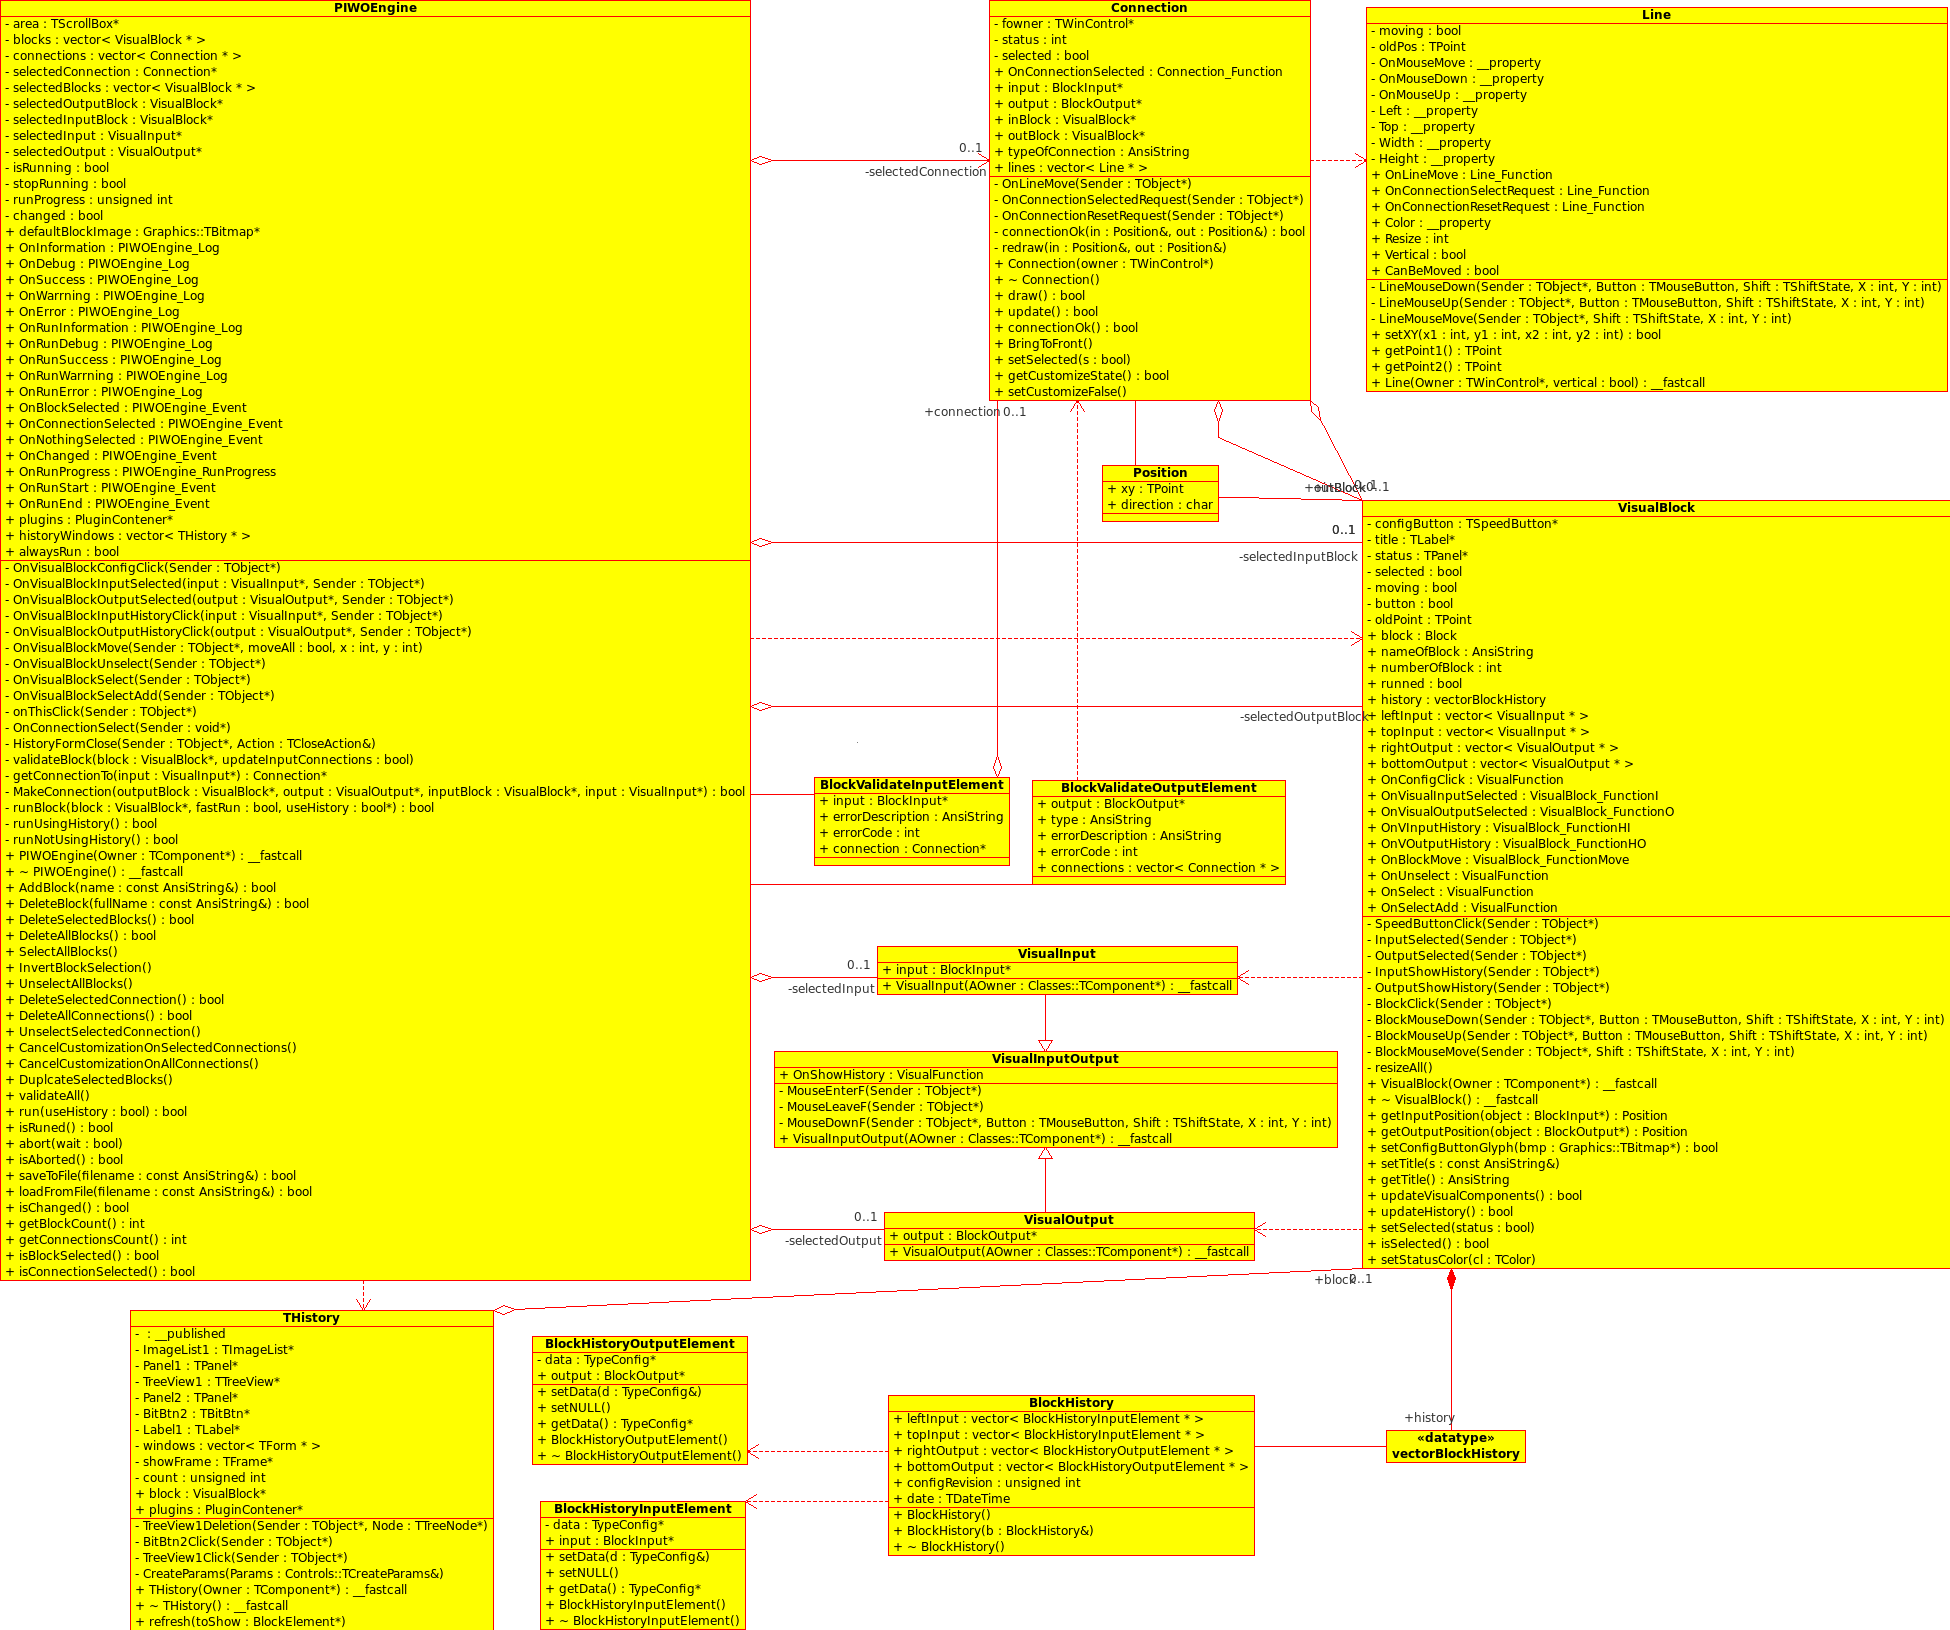
\includegraphics[scale=0.3]{diagram-gui.png}
 \caption{Engine - GUI}
 \label{fig:gui}
\end{figure}
\newpage
\section{Pluginy}
Program obsługuje 2 typy pluginów:
\begin{itemize}
\item pluginy typów
\item pluginy bloków
\end{itemize}
Pluginy typów dostarczją aplikacji obsługi nowych typów danych, aczkolwiek aplikacja i tak poprawnie uruchomi bloczki korzystające z niewspieranych typów, haczyk jest w tym że niekture opcje takie jak podgląd nie będą dostępne dla danego typu.
Informacje o typie danych są zapisywane w klasie TypeConfig.\\

Każda DLL pluginu jest ładowana do pamięci tylko RAZ.
Wymagania nałożone na każdą DLL pełniącą rolę pluginu:
\begin{itemize}
\item Każda DLL musi zawierać: \#pragma link ``MEMMGR.LIB''
\item Każda DLL musi być dostarczona w formie Release.
\item Każda DLL musi być skompilowana z opcją: Packages->Build with runtime packages(true) = vcl;rtl;vclx
\item Każda DLL musi być skompilowana z opcją: Linker->Linking->Use dynamic RTL = false
\end{itemize}
\subsection{Struktura DLL typu i wymagania}
Każda DLL typu musi powprawnie implementować i exportować następujące funkcje:\\
\textit{TFrame\* \_\_stdcall show(TWinControl\* owner, TypeConfig\* aData);}\\
Zadaniem tej funkcji jest poprawne wuświetlenie typu danych. Programista musi zaprojektować własną klase pochodną od TFrame na której w sposób wizualnie poprawny, nizależny od szerokości Frame ma wyświetlić dane zawarte w aData.Po poprawnym stworzeniu takiego obiektu narzucając mu owner który jest przesyłany w paametrze funkcji jak i Parent ma zwrócić wskaźnik do dopiero co utworzonego i wypełnionego danymi Frame.\\\\

\textit{bool \_\_stdcall isValid(TypeConfig\* aData);}\\
Zadaniem tej funkcji jest sprawdzenie poprawności typu. Funkcja musi sprawdzić typ aData, dane w nim zawartym, czy są poprawne i czy są odpowiedniego typu i zwrócić true w przypadku gdy typ jest poprawny, false gdy nie jest.\\\\
\textit{AnsiString \_\_stdcall getType();}\\
Funkcja ta ma tylko i wyłącznie zwrócić nazwę typu danych.

\subsection{Interfejsy typów}
Mianem interfejsu typu okresla się klasę z statycznymi metodami służacymi do tworzenia nowego typu pustego typu danych, zapisywania do niego i odczytywania z niego.
\subsection{Struktura DLL funkcji i wymagania}
W każdej z funkcji programista posiada pełną władze nad obiektem aBlock który symbolizuje blok.
Każda DLL funkcji musi implementować i eksportować następujące funkcje:\\
\textit{bool \_\_stdcall showConfig(TComponent \*owner, Block \*aBlock);}\\
Funkcja ta ma za zadanie pokazać okienko konfiguracyjne bloczka, po jej zakończeniu niemoże ona zostawiać aktywnego okna chyba że okno to jest powiązane z aBlock->blockWindow. Argument owner powinien być parentem i właścicielem nowo stworzonego okna. W interesie programującego jest zapewnić poprawne usunięcie okna z pamięci z wyjątkiem przypadku w którym okno jest powiązane z aBlock->blockWindow. Programista może tu zwrócić false w przypadku gdy niepotrzebuje aby bloczek miał okno konfiguracyjne, w innym przypadku powinien zwrócić true. Funkcja ta jest wywoływana tylko w przypadku gdy użytkownik jawnie kliknie w przycisk konfiguracyjny znajdujący się w centrum bloczka. Zabrania się odwołania do danych w tej funkcji, jak i modyfikacji wejść wyjść. Wszystkie dane które programista chce przechować powinny być przechowywane w klasie aBlock->getConfig().\\\\
\textit{int \_\_stdcall validate(Block \*aBlock);}
Funkcja ta jest wywoływana gdy:\\
\begin{itemize}
\item bloczek zostanie dodany do projektu
\item bloczek zostanie zduplikowany
\item zostanie dodane połączenie do bloczka (dotyczy tylko wejść)
\item zostanie usunięte połączenie do bloczka (dotyczy tylko wejść)
\item typ danych na dowolnym wejściu zostanie zmodyfikowany
\end{itemize}
\\
Funkcja powinna zwracać:\\
0 - gdy nie wprowadzono żadnych zmian w obiekcie aBlock\\
1 - gdy zmodyfikowano tylko kody błedów, opisy, typy danych\\
2 - gdy dodano nowe wejście / wyjście\\\\
W aktualnej wersji engine zwracany kod przez ta funkcje niema dużego wpływu na przetwarzanie projektu/bloku. Aczkolwiek w późniejszej wersji może to ulec zmianie, a poprawne zwracanie kodów może znacznie przyspieszyć działanie programu. Celem programisty w tej funkcji jest poprawne zarządzanie wejściami i wyjściami z bloku, inicjowanie konfiguracji. Programista ma nieograniczoną władzę nad wejsciami i wyjściami z bloku, może zarządzać typami danych jakie moga być podłączone do konkretnego wejścia, decydowac o typie danych jakie będzie dostarczone na wyjście i to właśnie tutaj musi o tym decydować. Kody błędów jakie wolno ustawić na wejściu / wyjściu to: 0 - wszystko ok, 1 - warrning. Kod 2- error jest zastrzeżony tylko i wyłącznie dla funkcji run.\\\\
\textit{int \_\_stdcall run(Block \*aBlock);}\\
Zadaniem funkcji jest wykonanie operacji ściśle powiązanej z bloczkiem. Jest to jedyna funkcja w której programista ma 100\% dostep do danych.\\\\
Kody wyjścia:\\
0 - wszystko ok\\
1 - warrning, coś nie zostało wykonane ale program może kontynuować\\
2 - error\\
\\
Programista w tej funkcji niemoże:\\
- dodawać, usuwać wejśc\\
- dodawać, usuwać wyjśc\\
- modyfikować typu danych na wyjściach\\
- modyfikować listy dozwolonych typów na wejściach\\
- odłączać połączenia podłączonego do wejścia\\
\\
Programista w tej funkcji ma obowiązek:\\
- poprawnie zwracać kody wyjść\\
- zwalniać pamięć po obiektach\\